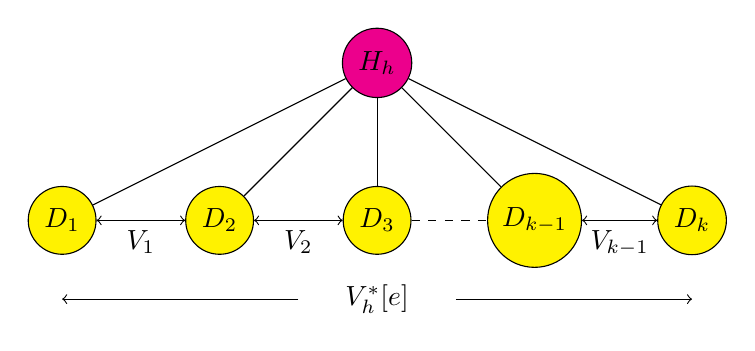
\begin{tikzpicture}

% Define the central node
\node[draw, circle, fill = magenta, minimum size=20pt] (H) at (0, 2) {$H_h$};

% Define the servant nodes along the x-axis
\node[draw, circle, fill = yellow] (node1) at (-4, 0) {$D_1$};
\node[draw, circle, fill = yellow] (node2) at (-2, 0) {$D_2$};
\node[draw, circle, fill = yellow] (node3) at (0, 0) {$D_3$};
\node[draw, circle, fill = yellow] (node1k) at (2, 0) {$D_{k-1}$};
\node[draw, circle, fill = yellow] (nodek) at (4, 0) {$D_{k}$};

% Connect servant nodes to the central node
\draw (H) -- (node1);
\draw (H) -- (node2);
\draw (H) -- (node3);
\draw (H) -- (node1k);
\draw (H) -- (nodek);

% Connect servant nodes to each other
\draw[<->] (node1) -- node[midway, below] {$V_1$} (node2) ;
\draw[<->] (node2) -- node[midway, below] {$V_2$} (node3) ;
\draw[dashed] (node3) -- (node1k);
\draw[<->] (node1k) -- node[midway, below] {$V_{k-1}$} (nodek);

\draw [->, ] (-1,-1) -- (-4,-1);

\draw [->, ] (1,-1) -- (4,-1);

\node at (0,-1){$V^*_h[e]$};

\end{tikzpicture}